% Grouped bar chart: Faith.-NLI and EM-F1 for all 12 conditions
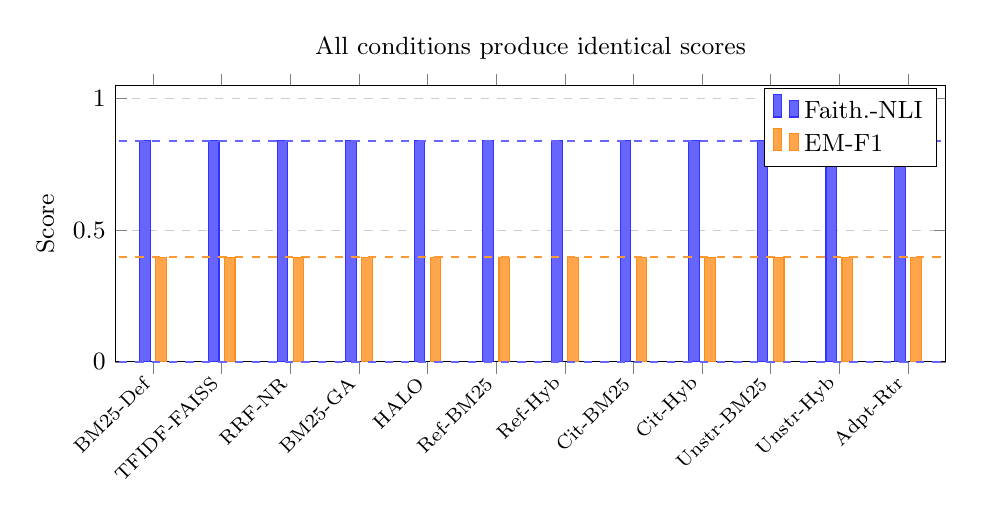
\begin{tikzpicture}
\begin{axis}[
  compat=1.18,
  ybar,
  bar width=3.8pt,
  width=\textwidth,
  height=0.42\textwidth,
  ymin=0, ymax=1.05,
  ylabel={Score},
  ylabel style={font=\small},
  title={\small All conditions produce identical scores},
  title style={font=\small},
  xtick={1,2,3,4,5,6,7,8,9,10,11,12},
  xticklabels={BM25-Def, TFIDF-FAISS, RRF-NR, BM25-GA, HALO,
               Ref-BM25, Ref-Hyb, Cit-BM25, Cit-Hyb,
               Unstr-BM25, Unstr-Hyb, Adpt-Rtr},
  x tick label style={font=\scriptsize, rotate=45, anchor=east},
  y tick label style={font=\small},
  legend style={at={(0.99,0.99)}, anchor=north east, font=\small,
                legend columns=1},
  legend cell align=left,
  ymajorgrids=true,
  grid style={dashed, gray!40},
  enlarge x limits=0.05,
  clip=false,
]

% Faith.-NLI bars (blue, value 0.84 for all 12 conditions)
\addplot[fill=blue!60, draw=blue!80] coordinates {
  (1,0.84) (2,0.84) (3,0.84) (4,0.84) (5,0.84) (6,0.84)
  (7,0.84) (8,0.84) (9,0.84) (10,0.84) (11,0.84) (12,0.84)
};
\addlegendentry{Faith.-NLI}

% EM-F1 bars (orange, value 0.3979 for all 12 conditions)
\addplot[fill=orange!70, draw=orange!90] coordinates {
  (1,0.3979) (2,0.3979) (3,0.3979) (4,0.3979) (5,0.3979) (6,0.3979)
  (7,0.3979) (8,0.3979) (9,0.3979) (10,0.3979) (11,0.3979) (12,0.3979)
};
\addlegendentry{EM-F1}

% Horizontal reference lines
\draw[dashed, blue!60, thick] ({rel axis cs:0,0} -| {axis cs:0.5,0})
  -- ({rel axis cs:1,0} -| {axis cs:12.5,0})
  node[right, font=\scriptsize, text=blue!70] {};
\draw[dashed, blue!60, thick] (axis cs:0.5, 0.84) -- (axis cs:12.5, 0.84);
\draw[dashed, orange!80, thick] (axis cs:0.5, 0.3979) -- (axis cs:12.5, 0.3979);

\end{axis}
\end{tikzpicture}
